% 2018 KTS
% Dancing links 패키지와 그 활용

\documentclass[xcolor=svgnames]{beamer}

\usetheme[titleformat=smallcaps,subsectionpage=progressbar]{metropolis}
\metroset{outer/progressbar=head}

\usepackage{fancyvrb}
\usepackage{kotex}
\hypersetup{pdfencoding=auto}

\usepackage{mathtools}
\usepackage{sudoku-dlx}
\usepackage{pentominoes}
\usepackage{queens}


% title
\title{Dancing links package}
\subtitle{Exact cover problem }
\date{2018년 2월 3일 토요일}
\author{남수진}
\institute{
  2018 한국텍학회 학술대회 및 정기총회 \\
  판교 스타트업캠퍼스 1동 2 층, 세미나실 1}
\titlegraphic{\hfill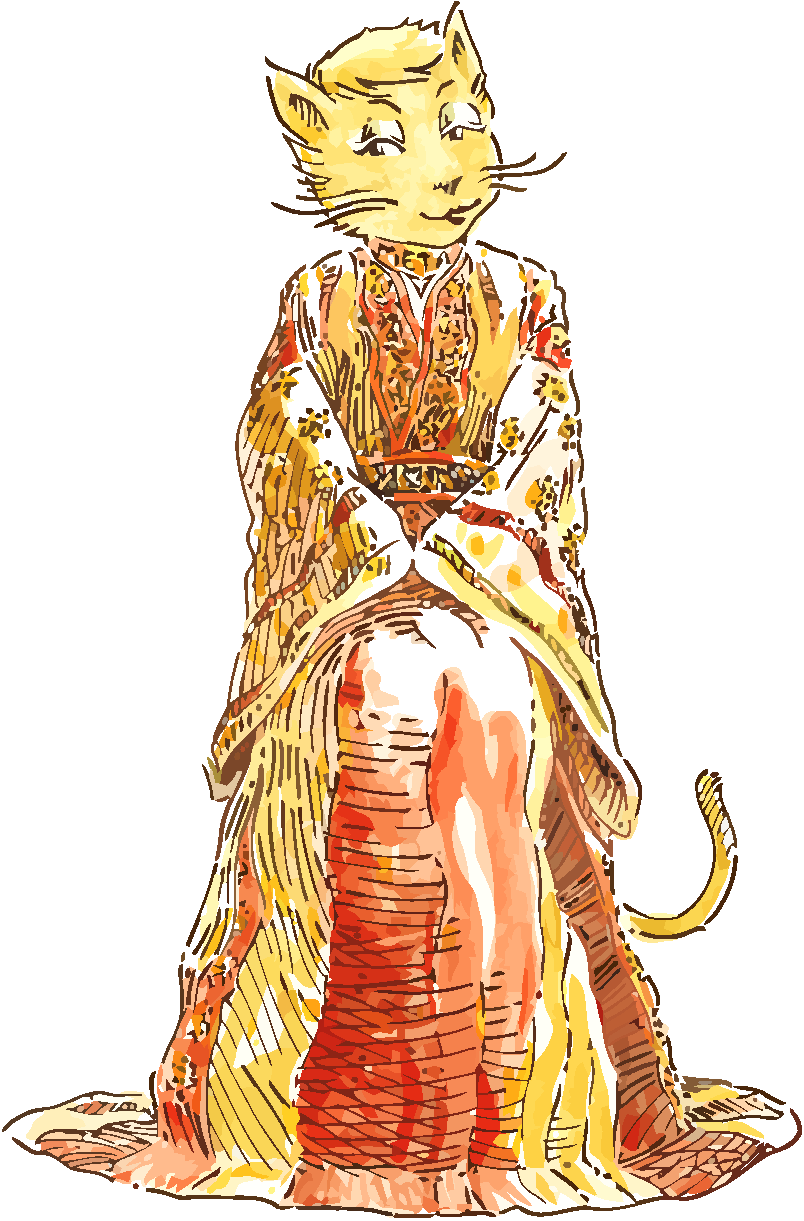
\includegraphics[height=3cm]{imgs/meta.pdf}}


%%
\begin{document}

\maketitle

%
\begin{frame}{Table of contents}
  \setbeamertemplate{section in toc}[sections numbered]
  \tableofcontents
\end{frame}

%%
\section{Dancing links}

%
\begin{frame}{Dancing links}
  \begin{itemize}
  \item Exact cover 문제를 해결하는 알고리즘에 사용되는 기법
  \item 백트래킹을 효율적으로 구현하는 방법 ($do$, $undo$ 연산)
  \end{itemize}
  \centering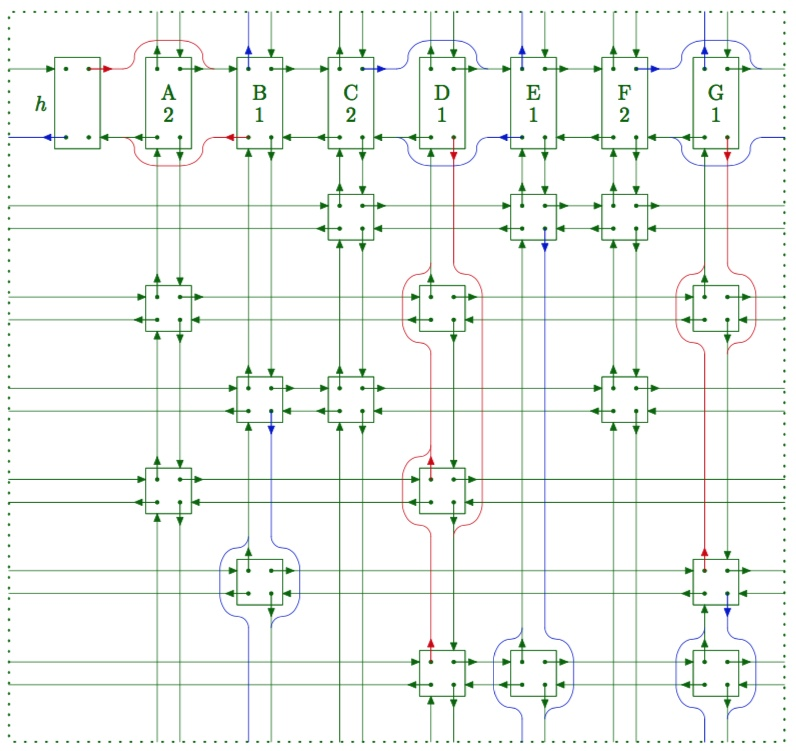
\includegraphics[height=6cm]{imgs/dlx.jpg}
\end{frame}

%%
\section{Exact cover problem}

%
\begin{frame}{Exact cover problem}
  0과 1로만 구성된 행렬에서 각 열이 정확히 하나의 1만 갖도록 하는
  행들의 집합을 구하라.
  $$
  \left(\begin{array}{ccccccc}
    0&0&1&0&1&0&0\\
    1&0&0&1&0&0&1\\
    0&1&1&0&0&1&0\\
    1&0&0&1&0&1&0\\
    0&1&0&0&0&0&1\\
    0&0&0&1&1&0&1
  \end{array}\right)
  $$
\end{frame}

\def\az{\alert0}
\def\ao{\alert1}
%
\begin{frame}{Exact cover problem}
  0과 1로만 구성된 행렬에서 각 열이 정확히 하나의 1만 갖도록 하는
  행들의 집합을 구하라.
  $$
  \left(\begin{array}{ccccccc}
    \az&\az&\ao&\az&\ao&\az&\az\\
    1&0&0&1&0&0&1\\
    0&1&1&0&0&1&0\\
    \ao&\az&\az&\ao&\az&\ao&\az\\
    \az&\ao&\az&\az&\az&\az&\ao\\
    0&0&0&1&1&0&1
    \end{array}\right)
$$
\end{frame}

%
\begin{frame}{Exact cover problem}
  \centering
  \begin{figure}[!htb]
    \begin{minipage}{.6\textwidth}
      \centering
      $\left(\begin{array}{ccccccc}
    0&0&1&0&1&0&0\\
    1&0&0&1&0&0&1\\
    0&1&1&0&0&1&0\\
    1&0&0&1&0&1&0\\
    0&1&0&0&0&0&1\\
    0&0&0&1&1&0&1
  \end{array}\right)\ \Rightarrow$
    \end{minipage}%
    \begin{minipage}{.4\textwidth}
      \centering
  $
  \begin{array}{ccccccc}
    A & B & C & D & E & F & G\\
    \hline
    C & E &&&&&\\
    A & D & G &&&&\\
    B & C & F &&&&\\
    A & D & F &&&&\\
    B & G &&&&&\\
    D & E & G &&&&
  \end{array}
  $
    \end{minipage}
\end{figure}
\end{frame}

\renewcommand\arraystretch{1.3}
%
\begin{frame}{Exact cover problem} 
  $$
  \begin{array}{ccccccc}
    A & B & C & D & E & F & G\\
    \hline
    C & E &&&&&\\
    A & D & G &&&&\\
    B & C & F &&&&\\
    A & D & F &&&&\\
    B & G &&&&&\\
    D & E & G &&&&
  \end{array}
  $$
\end{frame}

%
\begin{frame}{Exact cover problem} 
  $$
  \begin{array}{ccccccc}
    \alert A & B & C & \alert D & E & F & \alert G\\
    \hline
    C & E &&&&&\\
    \alert A & \alert D & \alert G &&&&\\
    B & C & F &&&&\\
    A & D & F &&&&\\
    B & G &&&&&\\
    D & E & G &&&&
  \end{array}
  $$
\end{frame}

%
\begin{frame}{Exact cover problem} 
  $$
  \begin{array}{ccccccc}
    \alert A & B & C & \alert D & E & F & \alert G\\
    \hline
    C & E &&&&&\\
    \alert A & \alert D & \alert G &&&&\\
    B & C & F &&&&\\
    &&&&&&\\
    &&&&&&\\
    &&&&&&
  \end{array}
  $$
\end{frame}

%
\begin{frame}{Exact cover problem} 
  $$
  \begin{array}{ccccccc}
    \alert A & B & \alert C & \alert D & \alert E & F & \alert G\\
    \hline
    \alert C & \alert E &&&&&\\
    \alert A & \alert D & \alert G &&&&\\
    B & C & F &&&&\\
    &&&&&&\\
    &&&&&&\\
    &&&&&&
  \end{array}
  $$
\end{frame}

%
\begin{frame}{Exact cover problem} 
  $$
  \begin{array}{ccccccc}
    \alert A & B & \alert C & \alert D & \alert E & F & \alert G\\
    \hline
    \alert C & \alert E &&&&&\\
    \alert A & \alert D & \alert G &&&&\\
    &&&&&&\\
    &&&&&&\\
    &&&&&&\\
    &&&&&&
  \end{array}
  $$
\end{frame}

%
\begin{frame}{Exact cover problem} 
  $$
  \begin{array}{ccccccc}
    \alert A & B & C & \alert D & E & \alert F & G\\
    \hline
    C & E &&&&&\\
    A & D & G &&&&\\
    B & C & F &&&&\\
    \alert A & \alert D & \alert F &&&&\\
    B & G &&&&&\\
    D & E & G &&&&
  \end{array}
  $$
\end{frame}

%
\begin{frame}{Exact cover problem} 
  $$
  \begin{array}{ccccccc}
    \alert A & B & C & \alert D & E & \alert F & G\\
    \hline
    C & E &&&&&\\
    &&&&&&\\
    &&&&&&\\
    \alert A & \alert D & \alert F &&&&\\
    B & G &&&&&\\
    &&&&&&
  \end{array}
  $$
\end{frame}

%
\begin{frame}{Exact cover problem} 
  $$
  \begin{array}{ccccccc}
    \alert A & B & \alert C & \alert D & \alert E & \alert F & G\\
    \hline
    \alert C & \alert E &&&&&\\
    &&&&&&\\
    &&&&&&\\
    \alert A & \alert D & \alert F &&&&\\
    B & G &&&&&\\
    &&&&&&
  \end{array}
  $$
\end{frame}

%
\begin{frame}{Exact cover problem} 
  $$
  \begin{array}{ccccccc}
    \alert A & \alert B & \alert C & \alert D
    & \alert E & \alert F & \alert G\\
    \hline
    \alert C & \alert E &&&&&\\
    &&&&&&\\
    &&&&&&\\
    \alert A & \alert D & \alert F &&&&\\
    \alert B & \alert G &&&&&\\
    &&&&&&
  \end{array}
  $$
\end{frame}

%
\begin{frame}{\texttt{lua-dancing-links}}
\vfill
\begin{center}
\Large
  \href{https://github.com/sjnam/lua-dancing-links}
    {github.com/sjnam/lua-dancing-links}
\end{center}
\vfill
\end{frame}

%%
\subsection{Pentominoes}

%
\begin{frame}[fragile]{Pentominoes}
\begin{verbatim}
\usepackage{pentominoes}
\pentominoes{1.4em}{3}{20}.
\end{verbatim}  

\pentominoes{1.4em}{3}{20}{1}.

\end{frame}

%
\begin{frame}{Pentominoes, 8x8}
\pentominoes{2em}{8}{8}{1}.
\end{frame}

%%
\subsection{Sudoku}

%
\begin{frame}[fragile]{Sudoku}
\begin{verbatim}
\sudoku {9.......6.3.4....9...915.8..8.5..7..%
..3.9.4....2..1.9.32176....6..1.2.3.8...5...1}
\end{verbatim}  

\begin{center}
  \sudoku{9.......6.3.4....9...915.8..8.5..7....3.9.4....2..1.9.32176....6..1.2.3.8...5...1}
\end{center}
\end{frame}

%
\begin{frame}[fragile]{Sudoku}
\begin{verbatim}
\sudoku*{9.......6.3.4....9...915.8..8.5..7..%
..3.9.4....2..1.9.32176....6..1.2.3.8...5...1}
\end{verbatim}

\begin{center}
  \sudoku*{9.......6.3.4....9...915.8..8.5..7....3.9.4....2..1.9.32176....6..1.2.3.8...5...1}
\end{center}
\end{frame}

%%
\subsection{N-Queens}

%
\begin{frame}[fragile]{n-queens}
\begin{verbatim}
\usepackage{queens}
\queens{8}{2}.
\end{verbatim}
\vspace{-10mm}
\queens{8}{2}.
\end{frame}

%
\begin{frame}{References}
  \begin{itemize}
  \item \href{http://www-cs-faculty.stanford.edu/~knuth/fasc5c.ps.gz}
    {\textsc{The Art of Computer Programming Pre-Fascicle 5c}}
  \item \href{https://github.com/sjnam/lua-dancing-links}
    {github.com/sjnam/lua-dancing-links}
  \end{itemize}
\end{frame}

%
\begin{frame}[standout]
  질문?
\end{frame}

\end{document}

